\documentclass[13pt,a4paper]{report}
\usepackage[utf8]{inputenc}
\usepackage[T5]{fontenc} % For Vietnamese
\usepackage[vietnamese]{babel}
\usepackage{amsmath}
\usepackage{amsfonts}
\usepackage{amssymb}
\usepackage{graphicx}
\usepackage[left=3cm,right=2cm,top=2cm,bottom=2cm]{geometry}
\usepackage{titlesec}
\usepackage{tocloft}
\usepackage{hyperref}
\usepackage{float}
\usepackage{tabularx}
\usepackage{caption}
\usepackage{chngcntr}
\usepackage{setspace}
\usepackage{microtype} % Giãn đều căn lề 2 bên
\usepackage{enumitem} % For custom lists
\usepackage{tikz}

% Kẻ khung báo cáo (Trang bìa)
\usepackage{pgf}
\usepackage{pgfpages}

% Hình đánh số theo chương giống sơ đồ
\counterwithin{figure}{chapter}
\counterwithin{table}{chapter}

% Căn lề đều 2 bên
\tolerance=1000
\emergencystretch=10pt
\hyphenpenalty=10000

% Thiết lập định dạng tiêu đề
\titleformat{\chapter}[display]
  {\normalfont\bfseries\Large\centering}{\chaptertitlename\ \thechapter}{10pt}{\LARGE}
\titlespacing*{\chapter}{0pt}{-20pt}{20pt}

% Các chương phải bắt đầu qua trang mới (Mặc định report class đã làm điều này)

\hypersetup{
    colorlinks=true,
    linkcolor=black,
    filecolor=magenta,      
    urlcolor=blue,
    pdftitle={Báo cáo Đồ án BusGIS},
}

\begin{document}

% ------------------- TRANG BÌA -------------------
\begin{titlepage}
\begin{tikzpicture}[remember picture, overlay]
  \draw[line width = 2pt] ($(current page.north west) + (3cm,-2cm)$) rectangle ($(current page.south east) + (-2cm,2cm)$);
  \draw[line width = 0.5pt] ($(current page.north west) + (3.1cm,-2.1cm)$) rectangle ($(current page.south east) + (-2.1cm,2.1cm)$);
\end{tikzpicture}

\begin{center}
    \vspace*{1cm}
    \Large \textbf{TRƯỜNG ĐẠI HỌC ...} \\
    \Large \textbf{KHOA CÔNG NGHỆ THÔNG TIN} \\
    \vspace{2cm}
    
    \includegraphics[width=4cm]{images/logo.png} % Hãy đảm bảo có logo hoặc xoá dòng này
    
    \vspace{2.5cm}
    \LARGE \textbf{BÁO CÁO ĐỒ ÁN} \\
    \vspace{1cm}
    \Huge \textbf{HỆ THỐNG WEBGIS QUẢN LÝ VÀ TRA CỨU TUYẾN XE BUÝT THÔNG MINH (BUSGIS)} \\
    \vspace{3cm}
    
    \Large
    \begin{tabular}{ll}
        \textbf{Giảng viên hướng dẫn:} & TS. Nguyễn Văn A \\
        \textbf{Sinh viên thực hiện:} & Lê Văn B \\
        \textbf{Mã số sinh viên:} & 12345678 \\
    \end{tabular}
    
    \vfill
    \Large TP. Hồ Chí Minh, \the\year
\end{center}
\end{titlepage}

% ------------------- MỤC LỤC -------------------
\tableofcontents
\listoffigures
\listoftables
\newpage

% ------------------- NỘI DUNG -------------------
\setstretch{1.3} % Giãn dòng 1.3

\chapter{TỔNG QUAN ĐỀ TÀI}

\section{Lý do chọn đề tài}

Trong bối cảnh đô thị hóa diễn ra mạnh mẽ và dân số tại các thành phố lớn tăng nhanh, vấn đề ùn tắc giao thông và ô nhiễm môi trường đang trở thành những thách thức cấp bách. Hệ thống giao thông công cộng, đặc biệt là mạng lưới xe buýt, đóng vai trò then chốt trong việc giải quyết các vấn đề này. Tuy nhiên, việc tra cứu thông tin tuyến xe, trạm dừng và lộ trình di chuyển tại nhiều thành phố hiện nay vẫn còn gặp nhiều hạn chế. Người dân thường gặp khó khăn trong việc tìm kiếm tuyến xe phù hợp, dẫn đến sự e ngại khi tiếp cận với phương tiện công cộng.

Bên cạnh đó, sự bùng nổ của công nghệ thông tin và bản đồ số đã mở ra những hướng đi mới trong việc quản lý và cung cấp dịch vụ hành khách. Hệ thống Thông tin Địa lý (GIS) kết hợp với nền tảng Web (WebGIS) cho phép trực quan hóa dữ liệu không gian một cách sinh động, cung cấp khả năng tra cứu trực tuyến và tương tác trực tiếp trên bản đồ. Các hệ thống hiện tại trên thị trường đôi khi giao diện chưa thân thiện, hoặc thiếu đi các tính năng phân tích không gian nâng cao như tìm trạm gần nhất theo bán kính hay đánh giá mức độ bao phủ của trạm.

Xuất phát từ những thực tiễn trên, việc nghiên cứu và xây dựng một nền tảng WebGIS hiện đại, tích hợp công cụ phân tích không gian mạnh mẽ là thực sự cần thiết. Đề tài "Hệ thống WebGIS quản lý và tra cứu tuyến xe buýt thông minh (BusGIS)" được lựa chọn nhằm cung cấp một giải pháp toàn diện. Hệ thống không chỉ hỗ trợ người dùng cuối dễ dàng tiếp cận thông tin mạng lưới xe buýt mà còn cung cấp cho nhà quản lý các công cụ để giám sát, đánh giá và quy hoạch luồng tuyến hiệu quả hơn.

Việc ứng dụng các công nghệ mã nguồn mở tiên tiến như Django, PostgreSQL/PostGIS và LeafletJS trong phát triển hệ thống cũng giúp tối ưu chi phí triển khai. Đây là cơ hội để vận dụng những kiến thức đã học vào thực tiễn, giải quyết một bài toán có ý nghĩa xã hội cao, góp phần thúc đẩy thói quen sử dụng giao thông công cộng hướng tới xây dựng thành phố thông minh và phát triển bền vững.

\section{Mục tiêu nghiên cứu}

Mục tiêu tổng quát của đề tài là xây dựng thành công ứng dụng WebGIS hỗ trợ việc tra cứu, định tuyến và quản lý mạng lưới xe buýt, đáp ứng yêu cầu xử lý dữ liệu không gian thời gian thực. Cụ thể, đề tài hướng đến các mục tiêu chi tiết sau:

\begin{itemize}
    \item Nghiên cứu và ứng dụng thành công các công nghệ WebGIS hiện đại (Django, PostGIS, Leaflet) vào bài toán quản lý giao thông.
    \item Xây dựng cơ sở dữ liệu không gian lưu trữ mạng lưới tuyến, trạm dừng xe buýt tối ưu cho việc truy vấn.
    \item Phát triển thuật toán định tuyến và tìm kiếm trạm gần nhất dựa trên tọa độ GPS của người dùng.
    \item Xây dựng giao diện tương tác thân thiện, trực quan, hỗ trợ hiển thị bản đồ mượt mà trên nhiều thiết bị.
    \item Cung cấp phân hệ quản trị hệ thống cho phép thêm, sửa, xóa tuyến/trạm và theo dõi phản hồi người dùng.
\end{itemize}

\section{Đối tượng và Phạm vi nghiên cứu}

\textbf{Đối tượng nghiên cứu:}
\begin{itemize}
    \item Hệ thống Thông tin Địa lý (GIS) và kiến trúc ứng dụng WebGIS.
    \item Các thuật toán phân tích không gian: tính toán khoảng cách (Haversine), tìm đường đi ngắn nhất, phân tích vùng đệm (Buffer).
    \item Mô hình quan hệ cơ sở dữ liệu không gian PostGIS.
    \item Nền tảng framework Django và thư viện hiển thị bản đồ LeafletJS.
\end{itemize}

\textbf{Phạm vi nghiên cứu:}
\begin{itemize}
    \item \textit{Phạm vi dữ liệu:} Tập trung thu thập, tiền xử lý và số hóa dữ liệu mạng lưới xe buýt tại khu vực Thành phố Hồ Chí Minh (dựa trên nguồn dữ liệu mở OpenStreetMap).
    \item \textit{Phạm vi chức năng:} Hệ thống giới hạn ở các chức năng tra cứu thông tin tuyến, trạm, định tuyến giữa hai điểm, quản lý dữ liệu, đăng ký tài khoản và đánh giá tuyến/trạm.
\end{itemize}

\section{Phương pháp nghiên cứu}

Để đạt được các mục tiêu đề ra, đề tài áp dụng các phương pháp nghiên cứu sau:

\begin{itemize}
    \item \textbf{Phương pháp nghiên cứu tài liệu:} Tìm hiểu các giáo trình, tài liệu học thuật và tài liệu kỹ thuật liên quan đến GIS, WebGIS, thiết kế cơ sở dữ liệu và kỹ thuật lập trình web.
    \item \textbf{Phương pháp phân tích và thiết kế hệ thống:} Khảo sát yêu cầu người dùng, mô hình hóa dữ liệu (ERD), thiết kế kiến trúc hệ thống và xây dựng biểu đồ Use Case, Sequence, Activity UML.
    \item \textbf{Phương pháp thực nghiệm:} Cài đặt môi trường, lập trình xây dựng ứng dụng (Coding), triển khai cơ sở dữ liệu không gian thực tế và tiến hành kiểm thử (Testing) để đánh giá độ chính xác của các thuật toán phân tích.
    \item \textbf{Phương pháp chuyên gia:} Tham khảo ý kiến và sự hướng dẫn của giảng viên để tinh chỉnh các chức năng, đảm bảo hệ thống bám sát các yêu cầu thực tiễn.
\end{itemize}

\chapter{CƠ SỞ LÝ THUYẾT VÀ DỮ LIỆU SỬ DỤNG}

\section{Hệ thống thông tin địa lý (GIS)}

Hệ thống thông tin địa lý (Geographic Information System - GIS) là hệ thống bao gồm phần cứng, phần mềm, dữ liệu không gian và các quy trình dùng để thu thập, lưu trữ, quản lý, thao tác, phân tích và hiển thị tất cả các dạng thông tin liên quan đến địa lý. Cốt lõi của GIS là khả năng gắn kết dữ liệu thuộc tính (thông tin dạng chữ, số) với dữ liệu không gian (tọa độ vị trí), cho phép người dùng hình dung, hiểu và diễn giải dữ liệu dưới nhiều hình thức trực quan như bản đồ trực tuyến, báo cáo và đồ thị. Trong quản lý giao thông, GIS đóng vai trò quan trọng trong việc theo dõi mạng lưới hạ tầng, quản lý tuyến xe, phân tích lưu lượng và hỗ trợ đưa ra quyết định tối ưu lộ trình. 

\section{Thuật toán Haversine – Tính khoảng cách địa lý}

Việc tính toán khoảng cách thực tế giữa hai điểm trên bề mặt Trái Đất không thể sử dụng hình học Euclid thông thường do bề mặt Trái Đất có độ cong hình cầu. Trong hệ thống BusGIS, để giải quyết bài toán tìm các trạm dừng nằm trong bán kính phục vụ (Buffer) hoặc đo lường khoảng cách trực tiếp giữa vị trí người dùng và trạm xe buýt gần nhất, hệ thống ứng dụng thuật toán Haversine. Thuật toán này xác định khoảng cách vòng lớn giữa hai điểm trên mặt cầu khi biết tọa độ kinh độ và vĩ độ của chúng.

Công thức Haversine được biểu diễn một cách chính xác theo phương trình sau:

\begin{equation}
    a = \sin^2\left(\frac{\Delta \varphi}{2}\right) + \cos(\varphi_1) \cdot \cos(\varphi_2) \cdot \sin^2\left(\frac{\Delta \lambda}{2}\right)
\end{equation}

\begin{equation}
    c = 2 \cdot \text{atan2}\left(\sqrt{a}, \sqrt{1-a}\right)
\end{equation}

\begin{equation}
    d = R \cdot c
\end{equation}

Trong đó:
\begin{itemize}
    \item $d$ là khoảng cách địa lý giữa hai điểm (đơn vị thường dùng là km hoặc mét).
    \item $R$ là bán kính trung bình của Trái Đất (tương đương khoảng $6,371$ km).
    \item $\varphi_1, \varphi_2$ lần lượt là vĩ độ của điểm thứ nhất và điểm thứ hai (tính bằng radian).
    \item $\Delta\varphi = \varphi_2 - \varphi_1$ là hiệu số vĩ độ giữa hai điểm.
    \item $\Delta\lambda = \lambda_2 - \lambda_1$ là hiệu số kinh độ giữa hai điểm (tính bằng radian).
\end{itemize}

Bằng việc áp dụng các phương trình trên vào hệ thống, quá trình truy vấn không gian diễn ra nhanh chóng, cho phép hiển thị khoảng cách với độ sai số cực thấp trên nền tảng WebGIS.

\section{WebGIS và Bản đồ trực tuyến}

WebGIS là sự kết hợp giữa kiến trúc mạng World Wide Web và Hệ thống thông tin địa lý, cho phép xử lý, phân tích và chia sẻ dữ liệu không gian thông qua trình duyệt web mà không cần cài đặt phần mềm chuyên dụng. Hệ thống hoạt động theo mô hình Client-Server, nơi máy chủ (Server) đảm nhận nhiệm vụ lưu trữ, truy vấn CSDL không gian và phản hồi kết quả, trong khi máy khách (Client) thực hiện hiển thị giao diện bản đồ, xử lý các tương tác của người dùng. Bản đồ trực tuyến cung cấp giao diện tương tác động, hỗ trợ các thao tác như thu phóng (zoom), di chuyển (pan) và hiển thị thông tin chi tiết qua các lớp dữ liệu (Layers), mang lại trải nghiệm người dùng tối ưu.

\section{Công nghệ sử dụng trong đồ án}

Để phát triển ứng dụng WebGIS quản lý xe buýt, đề tài kết hợp sử dụng các nền tảng công nghệ mạnh mẽ và mã nguồn mở. Toàn bộ logic nghiệp vụ phía máy chủ được phát triển bằng ngôn ngữ Python thông qua Web Framework Django. Việc sử dụng Django cung cấp kiến trúc Model-Template-View vững chắc, tích hợp sẵn các cơ chế bảo mật và giao diện quản trị mạnh mẽ. Thay vì sử dụng cơ sở dữ liệu quan hệ thông thường, hệ thống tích hợp PostgreSQL kết hợp cùng phần mở rộng không gian PostGIS, cho phép lưu trữ và truy vấn trực tiếp các đối tượng hình học như điểm, đường, vùng một cách tối ưu.

Bên cạnh đó, việc xây dựng giao diện tương tác phía người dùng được thực hiện thông qua ngôn ngữ HTML và CSS kết hợp với framework Bootstrap, đảm bảo hiển thị phản hồi nhanh (responsive) trên mọi kích thước màn hình. Đặc biệt, để biểu diễn dữ liệu bản đồ động, thư viện JavaScript LeafletJS được áp dụng. LeafletJS nổi bật với tính mỏng nhẹ, khả năng xử lý hình ảnh bản đồ raster và vector xuất sắc, đồng thời dễ dàng tích hợp các lớp bản đồ cơ sở (basemaps) từ các dịch vụ bản đồ bên thứ ba.

\section{Nguồn dữ liệu và Tiền xử lý}

Toàn bộ dữ liệu phục vụ quá trình nghiên cứu và xây dựng hệ thống BusGIS được khai thác từ kho dữ liệu mở OpenStreetMap. Đây là một dự án bản đồ thế giới mở, cung cấp nguồn dữ liệu không gian phong phú được đóng góp bởi cộng đồng toàn cầu. Thông qua các công cụ truy xuất như Overpass API, hệ thống thu thập được hệ tọa độ chi tiết của các trạm dừng cũng như mảng tọa độ vẽ lộ trình của các tuyến xe buýt đang hoạt động tại khu vực Thành phố Hồ Chí Minh. Dữ liệu thô tải về mang định dạng chuẩn GeoJSON, chứa đầy đủ các thuộc tính không gian và phi không gian cần thiết.

Sau khi thu thập, quy trình tiền xử lý được thực hiện nhằm tinh gọn và đồng nhất hóa dữ liệu trước khi đưa vào cơ sở dữ liệu. Quá trình này bao gồm việc loại bỏ các thuộc tính không cần thiết, chuẩn hóa định dạng văn bản cho tên tuyến và địa chỉ, đồng thời chuyển đổi cấu trúc mạng tuyến thành danh sách tọa độ sắp xếp theo trình tự di chuyển hợp lý. Dữ liệu sau khi xử lý được chuyển đổi sang chuẩn WKT (Well-Known Text) và nạp trực tiếp vào các bảng PostGIS, sẵn sàng cho các thao tác phân tích truy vấn không gian trên giao diện WebGIS.

\chapter{PHÂN TÍCH VÀ THIẾT KẾ HỆ THỐNG}

\section{Kiến trúc hệ thống}

Kiến trúc hệ thống BusGIS được xây dựng dựa trên mô hình ba lớp (Three-tier Architecture) nhằm đảm bảo tính phân tách rõ ràng giữa các thành phần, tối ưu hóa hiệu suất và nâng cao khả năng mở rộng trong tương lai. Sự phân tách này không chỉ giúp cho quá trình bảo trì mã nguồn trở nên thuận tiện mà còn tăng cường mức độ bảo mật cho dữ liệu hệ thống.

Cụ thể, hệ thống bao gồm ba tầng chức năng chính:
\begin{itemize}
    \item \textbf{Tầng Trình diễn (Presentation Layer - Frontend):} Đây là giao diện tương tác trực tiếp với người sử dụng, được xây dựng dựa trên HTML, CSS và framework Bootstrap kết hợp với thư viện LeafletJS. Tầng này chịu trách nhiệm thu nhận yêu cầu của người dùng, chẳng hạn như thao tác tìm kiếm tuyến đường, chọn trạm dừng hoặc thao tác kéo thả trên bản đồ. Sau khi hệ thống xử lý, tầng trình diễn nhận kết quả phản hồi dưới dạng JSON và vẽ lại các lớp bản đồ không gian một cách trực quan. Việc sử dụng LeafletJS giúp giao diện thao tác nhanh chóng, giảm tải băng thông so với việc tải lại toàn bộ trang web.
    \item \textbf{Tầng Xử lý Logic (Business Logic Layer - Backend):} Được phát triển hoàn toàn trên nền tảng Django (Python), tầng này đóng vai trò như bộ não của toàn bộ hệ thống. Nhiệm vụ chính của tầng xử lý logic là tiếp nhận các request từ phía người dùng, tiến hành xử lý nghiệp vụ xác thực, phân quyền và triển khai các thuật toán phân tích không gian phức tạp. Khi có yêu cầu tìm đường hoặc xác định bán kính vùng đệm, Backend sẽ chuyển hóa yêu cầu thành các câu lệnh truy vấn không gian phức hợp, kết nối với cơ sở dữ liệu để lấy kết quả và trả về cho Frontend dưới chuẩn API RESTful.
    \item \textbf{Tầng Dữ liệu (Data Access Layer - Database):} Đóng vai trò cốt lõi trong việc quản lý và duy trì tính toàn vẹn của thông tin. Tầng này sử dụng hệ quản trị cơ sở dữ liệu PostgreSQL kết hợp cùng phần mở rộng PostGIS. Sự kết hợp này mang đến khả năng lưu trữ không chỉ các trường dữ liệu văn bản truyền thống mà còn lưu trữ cấu trúc hình học phức tạp (Point, LineString). PostGIS hỗ trợ việc đánh chỉ mục không gian (Spatial Indexing) bằng cấu trúc R-Tree, giúp các tác vụ truy xuất dữ liệu bản đồ diện rộng được thực thi với tốc độ chỉ tính bằng mili-giây.
\end{itemize}

Sự kết hợp đồng bộ giữa ba tầng kiến trúc trên đã tạo ra một hệ thống WebGIS hoàn chỉnh, hoạt động xuyên suốt từ bước thu nhận yêu cầu của người dùng đến lúc truy xuất, tính toán số liệu và trả về kết quả đồ họa trên giao diện.

\section{Luồng dữ liệu (Data Flow / Pipeline)}

Quá trình luân chuyển dữ liệu bên trong hệ thống BusGIS được thiết kế một cách khoa học nhằm kiểm soát chặt chẽ trạng thái vòng đời của thông tin, từ giai đoạn thu thập ban đầu cho đến khi được biểu diễn trực quan trên bản đồ. Luồng xử lý dữ liệu được chia thành nhiều quy trình nối tiếp nhau, đảm bảo dữ liệu luôn đạt tiêu chuẩn đầu vào của hệ quản trị cơ sở dữ liệu.

Quy trình luân chuyển dữ liệu được thực hiện qua các bước chi tiết sau:
\begin{itemize}
    \item \textbf{Thu thập và Trích xuất dữ liệu thô:} Dữ liệu ban đầu về các tuyến xe buýt và điểm dừng được trích xuất từ cộng đồng bản đồ mở OpenStreetMap bằng cú pháp truy vấn Overpass QL. Dữ liệu trả về thường ở định dạng JSON dạng thô, mang theo rất nhiều thẻ (tags) dư thừa không cần thiết cho ứng dụng.
    \item \textbf{Tiền xử lý và Làm sạch (Data Cleansing):} Tại giai đoạn này, các tập lệnh Python (Scripts) sẽ duyệt qua bộ dữ liệu thô. Quá trình làm sạch tập trung vào việc loại bỏ các node không chứa thông tin quan trọng, chuẩn hóa tên tuyến xe, xử lý các ký tự đặc biệt trong địa chỉ trạm dừng và định dạng lại cấu trúc mảng tọa độ. Dữ liệu sau đó được định hình lại theo chuẩn GeoJSON với cấu trúc phân cấp thống nhất.
    \item \textbf{Chuyển đổi và Lưu trữ (Transform \& Load):} Từ tập dữ liệu GeoJSON đã làm sạch, Django ORM tiến hành chuyển đổi các cặp kinh độ, vĩ độ thành đối tượng hình học dạng điểm (Point) và chuỗi đường (LineString) tuân thủ hệ tọa độ WGS84 (SRID 4326). Dữ liệu này sau đó được ánh xạ trực tiếp vào các bảng quan hệ trong PostGIS, đồng thời tạo ra các mối liên kết khóa ngoại (Foreign Keys) giữa bảng Tuyến, bảng Trạm và bảng trung gian (RouteStop).
    \item \textbf{Truy vấn và Phân tích (Query \& Analysis):} Khi có yêu cầu tương tác từ người dùng (như nhấn chọn xem chi tiết tuyến), hệ thống thực hiện lệnh truy vấn SQL thông qua Django ORM. Dữ liệu được trích xuất từ cơ sở dữ liệu, đi qua các bộ lọc và hàm phân tích không gian (nếu có), sau đó đóng gói thành định dạng JSON.
    \item \textbf{Hiển thị trực quan (Visualization):} Frontend nhận gói dữ liệu JSON từ Backend, sử dụng các hàm API của LeafletJS để vẽ đối tượng lên không gian bản đồ. Các điểm (Markers) biểu thị cho trạm dừng, các đường gấp khúc (Polylines) biểu thị cho lộ trình di chuyển. Mỗi đối tượng đều được đính kèm các popup hiển thị thông tin chi tiết.
\end{itemize}

\section{Thiết kế cơ sở dữ liệu}

Cơ sở dữ liệu của BusGIS được thiết kế đảm bảo các chuẩn mực chuẩn hóa, giảm thiểu tối đa hiện tượng dư thừa dữ liệu và hỗ trợ đắc lực cho các liên kết không gian. 

\begin{figure}[H]
    \centering
    
\includegraphics[width=\textwidth]{images/image1.png}
    \caption{Mô hình thực thể kết nối (ERD) tổng quan}
\end{figure}

Dữ liệu được chia thành các bảng chính bao gồm:
\begin{itemize}
    \item \textbf{Bảng BusRoute:} Lưu trữ thông tin chi tiết của tuyến xe như số hiệu tuyến, tên tuyến, điểm đầu, điểm cuối, thời gian hoạt động, giá vé và màu sắc hiển thị trên bản đồ.
    \item \textbf{Bảng BusStop:} Lưu trữ vị trí không gian của các trạm xe buýt. Điểm nổi bật là trường vị trí được cấu hình kiểu hình học \texttt{Point(Lon, Lat)} để truy vấn khoảng cách. Ngoài ra còn lưu thông tin mã trạm, tên trạm, địa chỉ và các tiện ích đi kèm (mái che, ghế ngồi).
    \item \textbf{Bảng RouteStop (Trung gian):} Quản lý mối quan hệ nhiều - nhiều giữa Tuyến và Trạm. Bảng này không chỉ liên kết khóa ngoại mà còn lưu trữ trường Thứ tự (Order) nhằm xác định hướng di chuyển chính xác của tuyến xe.
    \item \textbf{Bảng User và UserProfile:} Quản lý tài khoản người dùng, lưu trữ thông tin xác thực, phân quyền hệ thống (User, Staff, Admin) và các thông tin liên hệ.
    \item \textbf{Bảng Review:} Cho phép người dùng đánh giá và phản hồi về tuyến xe buýt hoặc trạm dừng, bao gồm điểm số đánh giá và nội dung nhận xét.
\end{itemize}

\section{Thiết kế chức năng (Use Case)}

Hệ thống BusGIS cung cấp đa dạng các chức năng đáp ứng nhu cầu cho hai nhóm đối tượng chính: Người dùng khách (Guest/User) và Quản trị viên (Admin/Staff).

\begin{figure}[H]
    \centering
    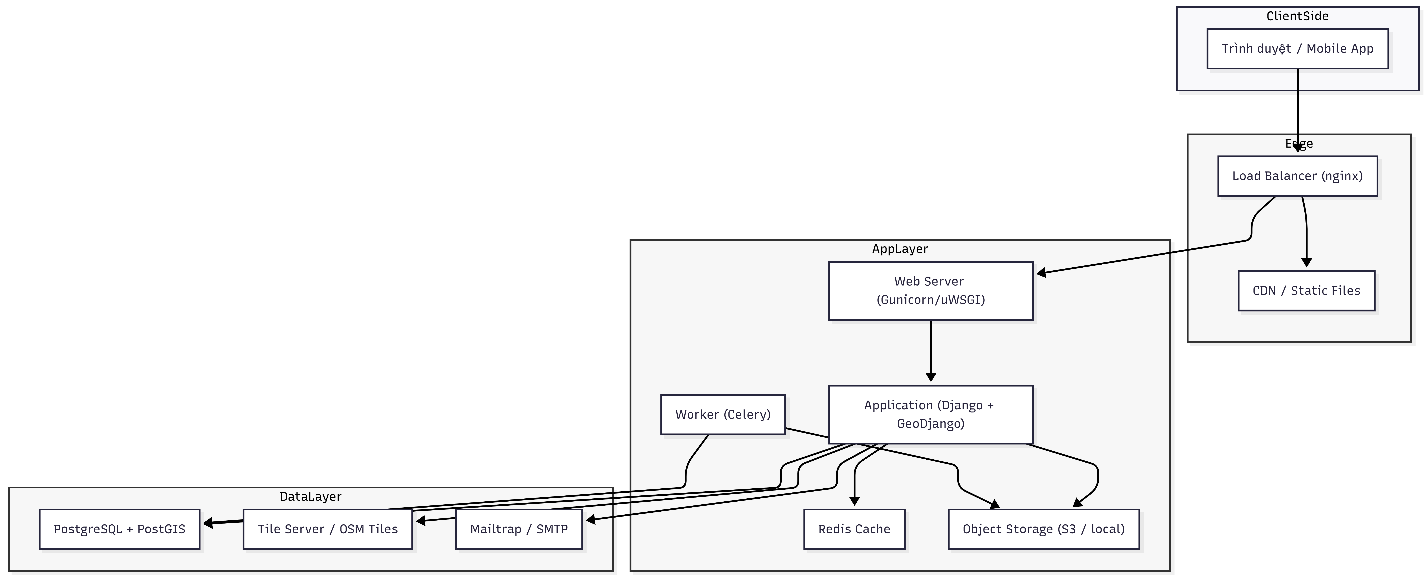
\includegraphics[width=\textwidth]{images/image2.png}
    \caption{Sơ đồ Use Case tổng quát hệ thống}
\end{figure}

Các chức năng chính được phân chia theo từng vai trò như sau:
\begin{itemize}
    \item \textbf{Nhóm chức năng dành cho Người dùng:}
    \begin{itemize}
        \item Tra cứu tuyến xe buýt, xem chi tiết đường đi, điểm đầu cuối, giá vé.
        \item Tìm kiếm trạm dừng, xác định vị trí trạm trên bản đồ và tiện ích tại trạm.
        \item Đăng ký tài khoản, đăng nhập và quản lý thông tin hồ sơ cá nhân.
        \item Sử dụng các công cụ GIS nâng cao: Tìm tuyến đường theo tọa độ hiện tại, tìm trạm dừng trong phạm vi bán kính cho trước.
        \item Gửi đánh giá, nhận xét trải nghiệm sử dụng đối với từng tuyến xe hoặc trạm dừng.
    \end{itemize}
    
    \item \textbf{Nhóm chức năng dành cho Quản trị viên:}
    \begin{itemize}
        \item Quản trị toàn diện mạng lưới dữ liệu xe buýt (Thêm, Sửa, Xóa mềm đối với Tuyến xe và Trạm dừng).
        \item Import và Export dữ liệu hàng loạt từ các định dạng Excel, hỗ trợ cập nhật thông tin nhanh chóng.
        \item Quản lý tài khoản người dùng, theo dõi trạng thái hoạt động và phân quyền nhân viên.
        \item Theo dõi và kiểm duyệt các đánh giá (Reviews) từ người dùng đối với các dịch vụ.
        \item Truy cập bảng thống kê trực quan (Dashboard) hiển thị tổng quan số lượng tuyến, trạm và lưu lượng tương tác của hệ thống.
    \end{itemize}
\end{itemize}

Để làm rõ chi tiết nghiệp vụ thao tác, các quy trình cốt lõi được biểu diễn thông qua Sơ đồ Tuần tự (Sequence Diagram) và Sơ đồ Hoạt động (Activity Diagram).

\begin{figure}[H]
    \centering
    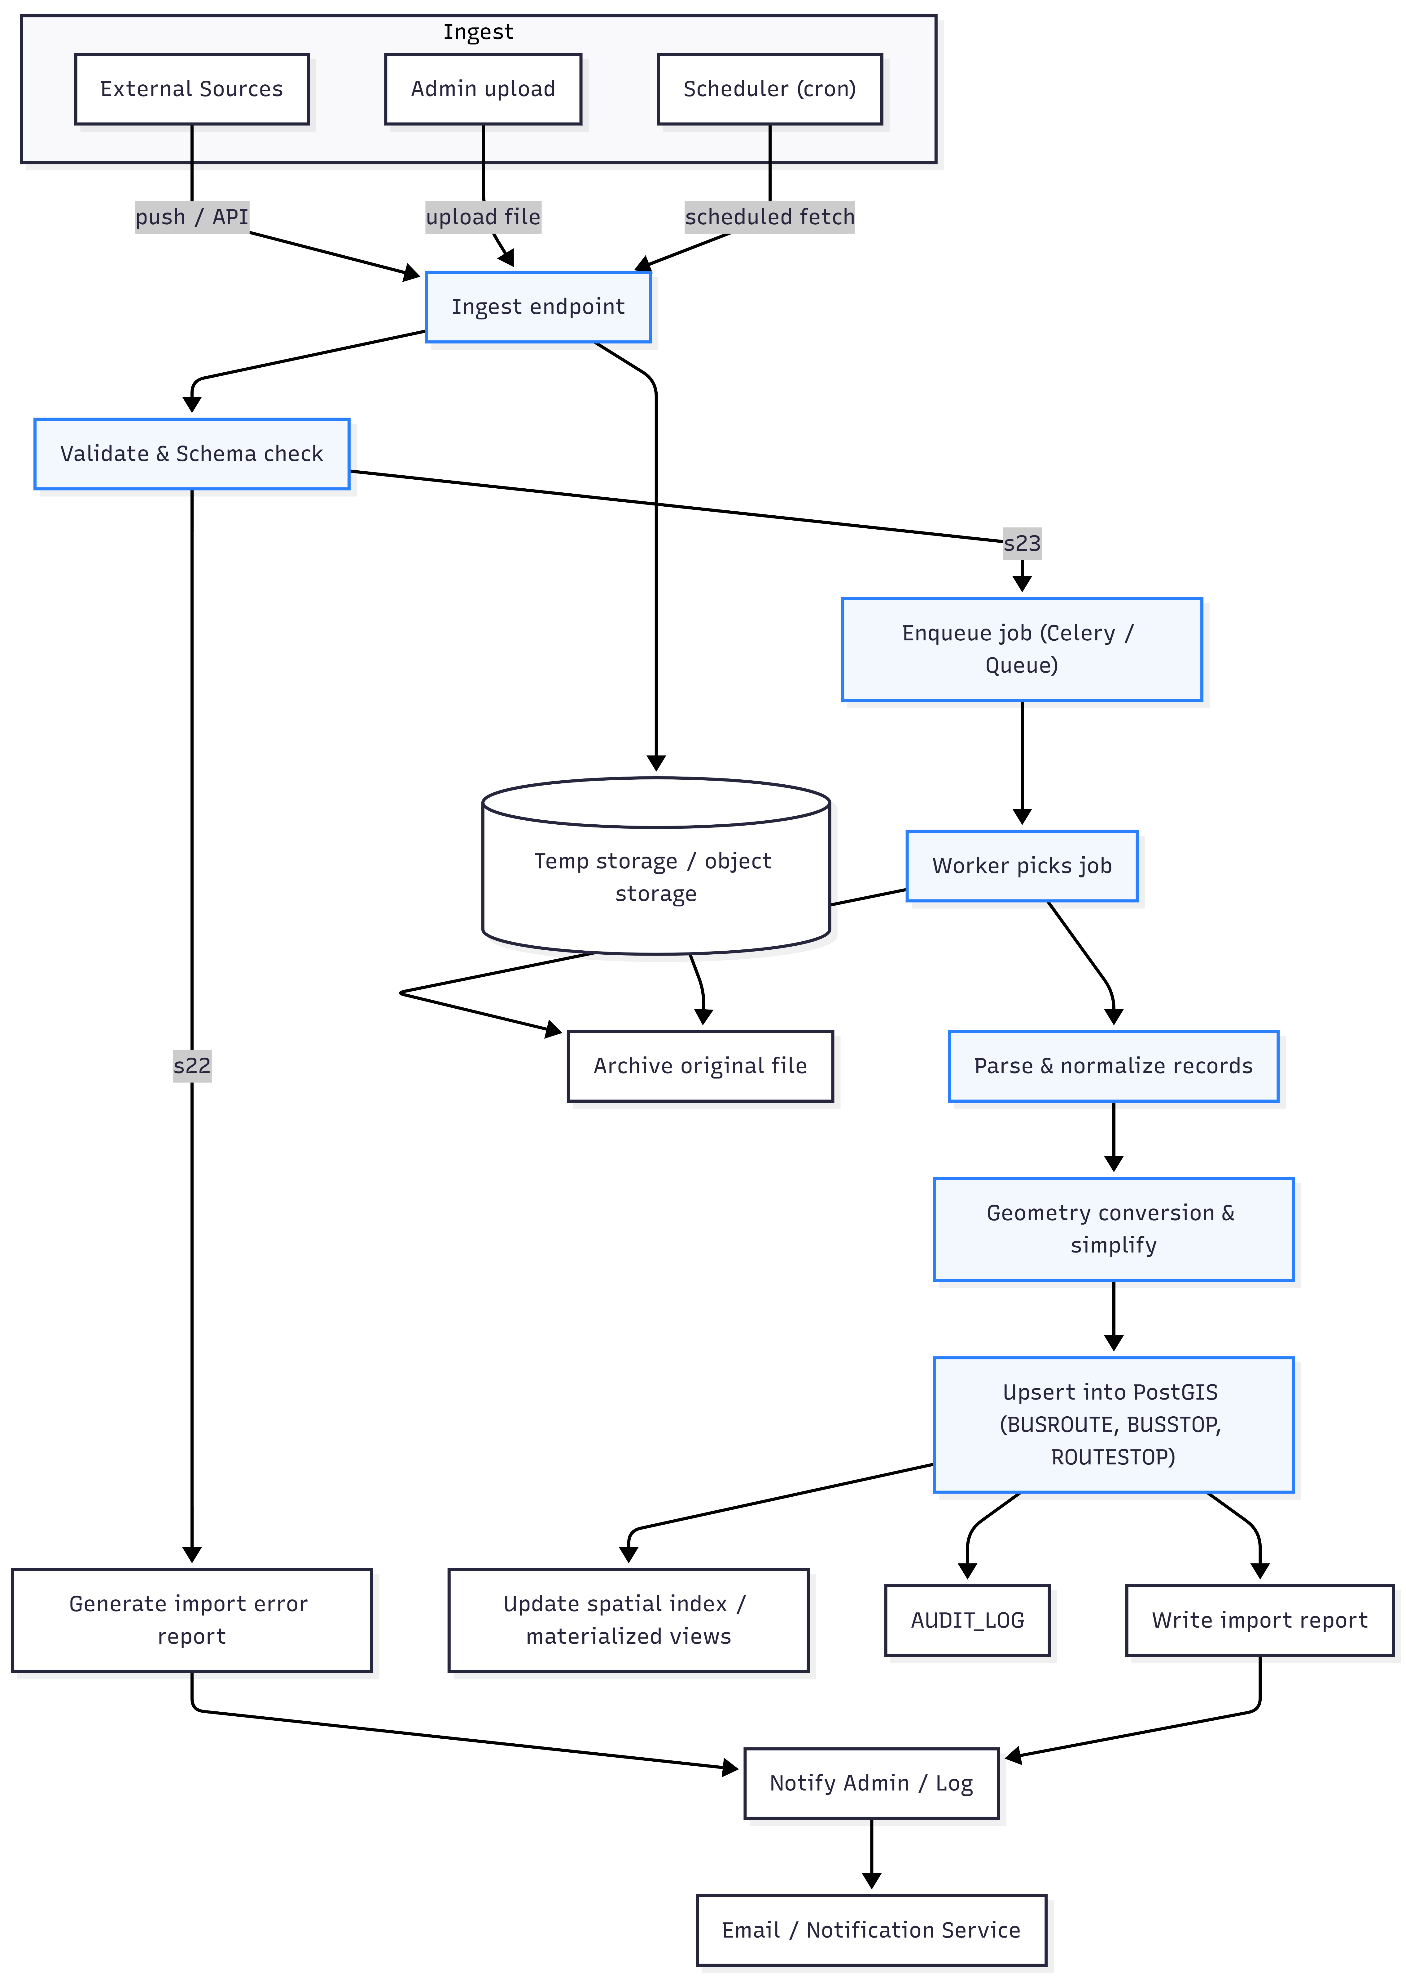
\includegraphics[width=\textwidth]{images/image3.png}
    \caption{Sơ đồ hoạt động quy trình tìm kiếm và định tuyến}
\end{figure}

Sơ đồ trên minh họa quá trình người dùng nhập điểm bắt đầu và kết thúc, hệ thống sẽ giao tiếp với máy chủ PostGIS để tính toán thuật toán khoảng cách và phản hồi danh sách các tuyến phù hợp để biểu diễn lên bản đồ trực quan.

\chapter{KẾT QUẢ TRIỂN KHAI VÀ XÂY DỰNG WEBSITE}

\section{Phân hệ giao diện tương tác Người dùng (Guest Web UI)}

\subsection{Trang Giới thiệu hệ thống (Landing Page)}

Trang Landing Page đóng vai trò là cửa ngõ đầu tiên chào đón người dùng truy cập vào BusGIS. Giao diện được thiết kế theo phong cách hiện đại, sử dụng hiệu ứng chuyển động mượt mà (animations) và bố cục hiển thị trực quan. Ngay từ trang chủ, hệ thống cung cấp bản đồ demo nhỏ để minh họa cho khả năng theo dõi lộ trình tuyến xe.

\begin{figure}[H]
    \centering
    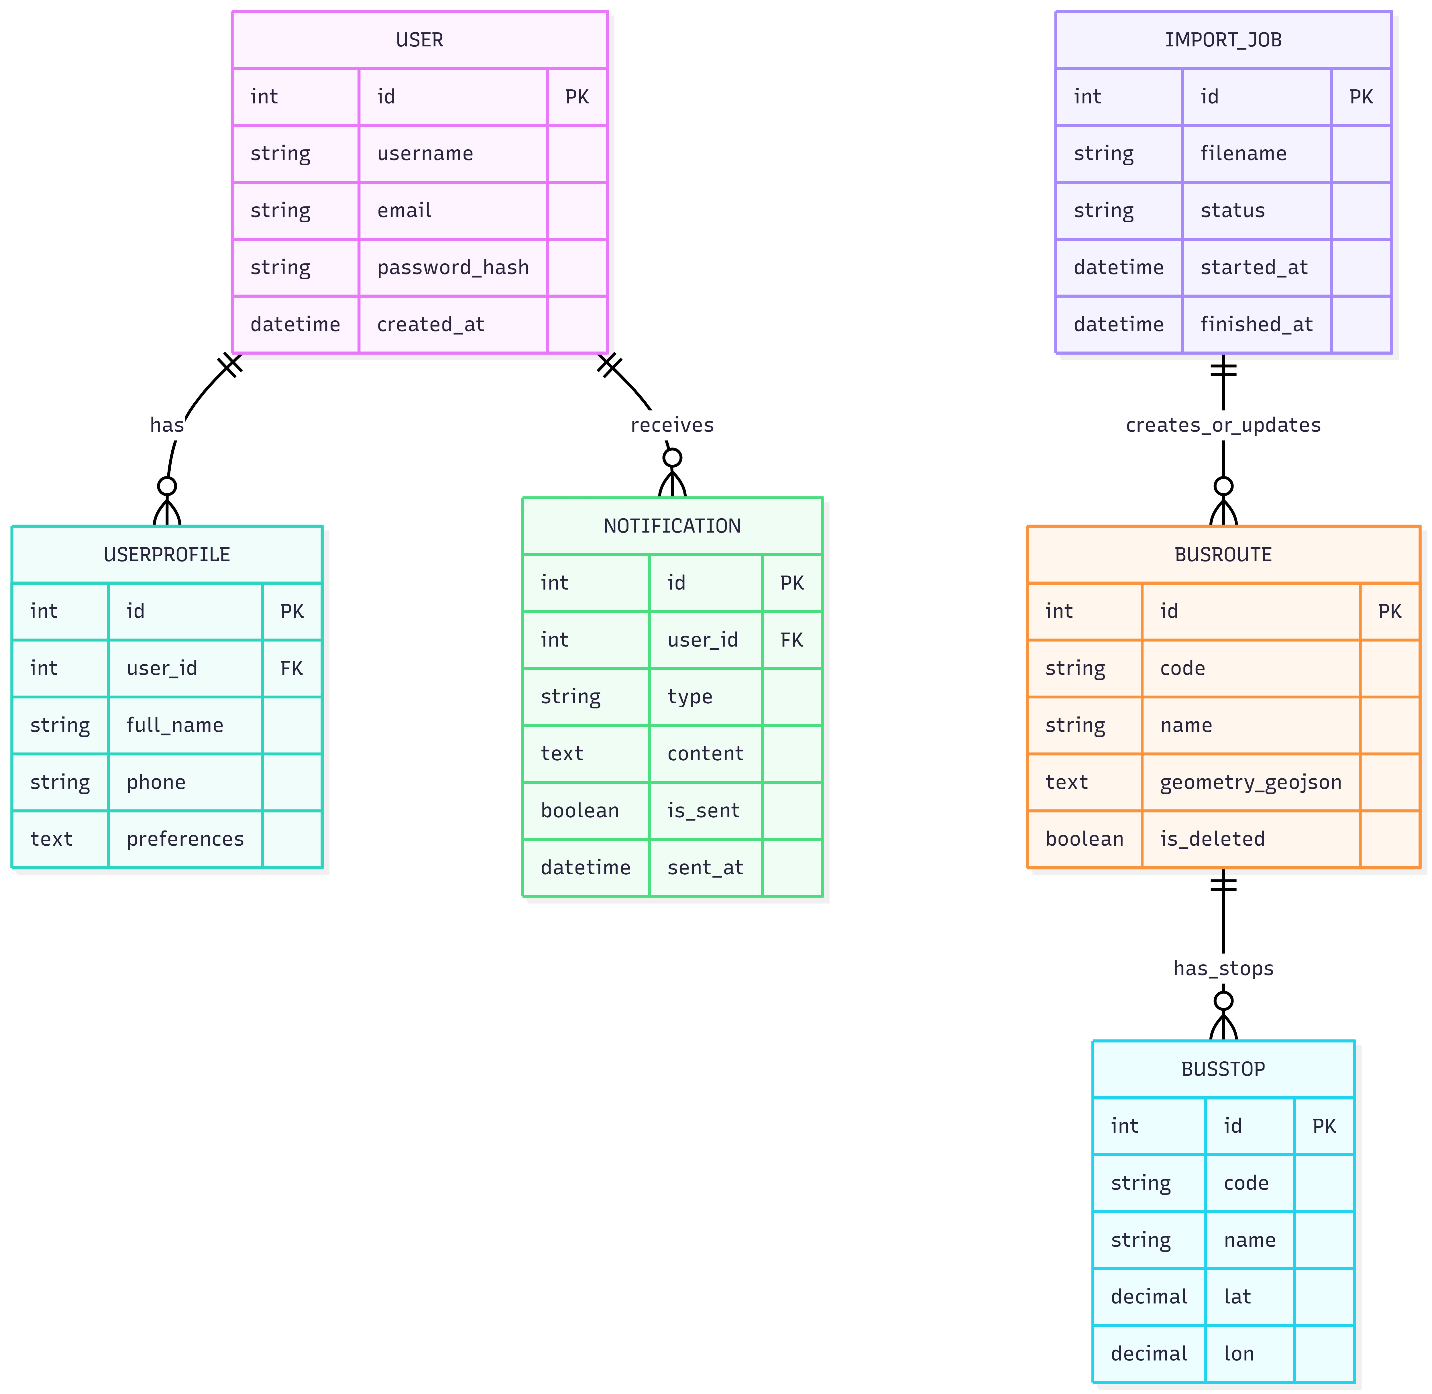
\includegraphics[width=\textwidth]{images/image4.png}
    \caption{Giao diện Trang giới thiệu hệ thống (Landing Page)}
\end{figure}

Trang cung cấp thông tin tóm tắt về số lượng tuyến, trạm hiện có và mô tả các tính năng nổi bật. Tùy thuộc vào trạng thái xác thực, hệ thống sẽ điều hướng người dùng đăng nhập hoặc truy cập trực tiếp vào hệ thống bản đồ lõi.

\subsection{Giao diện Trang chủ và nền tảng Bản đồ số}

Trung tâm của ứng dụng là Trang chủ chứa Bản đồ số tích hợp. Giao diện bản đồ được xây dựng dựa trên LeafletJS chiếm toàn bộ không gian khung hình, mang lại cảm giác trải nghiệm không giới hạn (Infinite Map View). 

\begin{figure}[H]
    \centering
    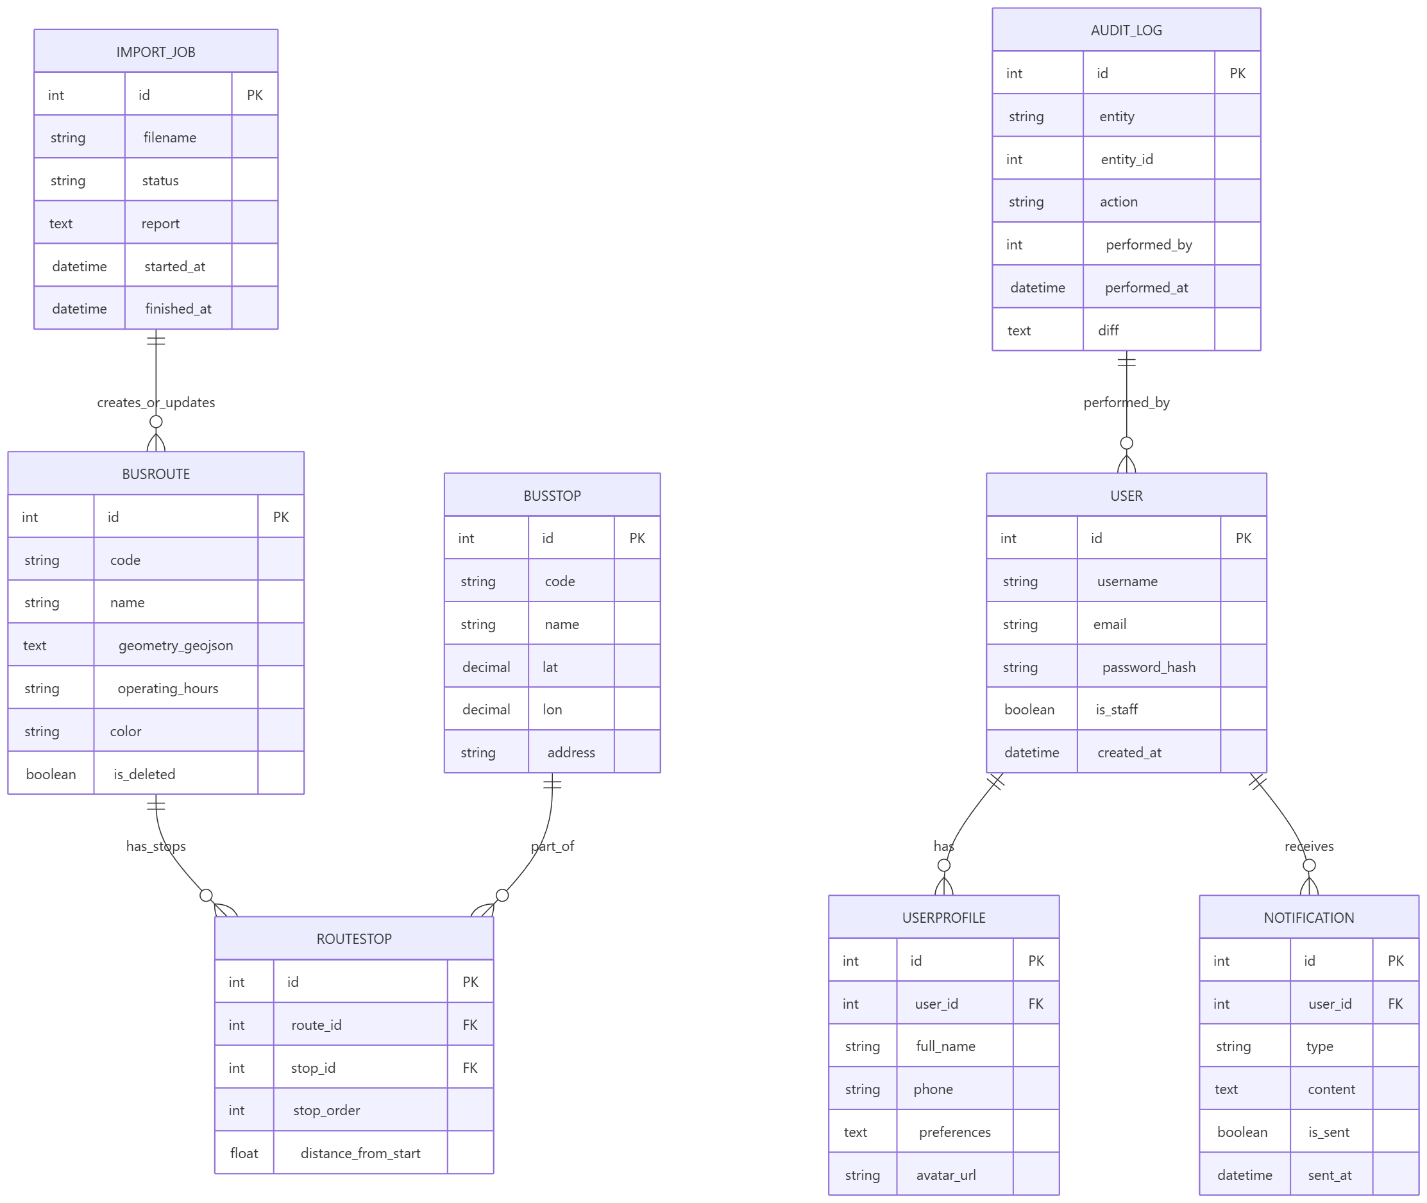
\includegraphics[width=\textwidth]{images/image5.png}
    \caption{Giao diện Trang chủ Bản đồ tương tác}
\end{figure}

Tại đây, người dùng có thể kéo thả, phóng to, thu nhỏ và nhấn chọn trực tiếp vào các biểu tượng điểm dừng (Markers) để xem tên trạm, địa chỉ. Hệ thống cũng cung cấp thanh tìm kiếm nhanh để xác định ngay vị trí một địa điểm cụ thể trên bản đồ.

\subsection{Danh mục truy xuất Tuyến xe buýt và Trạm dừng}

Tính năng truy xuất tuyến xe cho phép liệt kê toàn bộ mạng lưới xe buýt dưới dạng danh sách các thẻ thông tin (Cards). Mỗi thẻ hiển thị rõ ràng số tuyến, tên điểm đầu cuối và nhãn trạng thái hoạt động.

\begin{figure}[H]
    \centering
    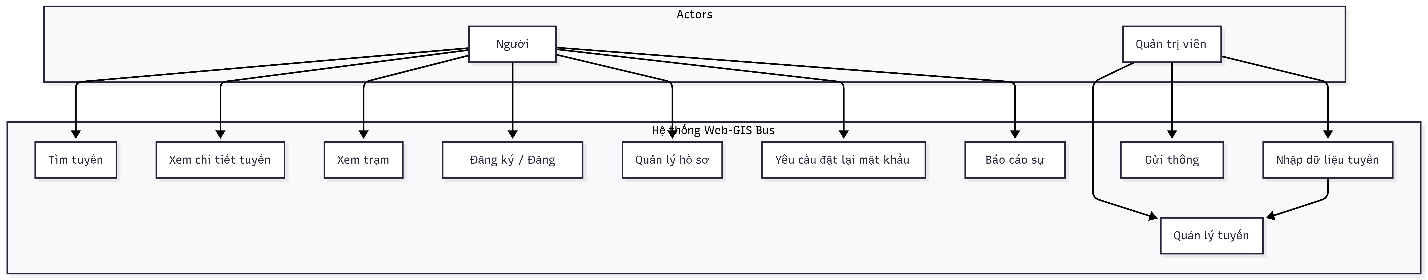
\includegraphics[width=\textwidth]{images/image6.png}
    \caption{Giao diện Danh sách các tuyến xe buýt}
\end{figure}

Giao diện còn hỗ trợ phân trang (Pagination) để tối ưu thời gian tải trang đối với các danh sách dài. Đối với danh sách Trạm dừng, người dùng có thể áp dụng các bộ lọc tiện ích như "Có mái che", "Có ghế ngồi" để sàng lọc kết quả hiển thị mong muốn.

\subsection{Chi tiết thông tin cấu trúc một Tuyến xe cụ thể}

Khi người dùng nhấn chọn một tuyến xe, hệ thống sẽ chuyển hướng sang Trang Chi tiết Tuyến. Tại đây, toàn bộ thông tin giá vé, thời gian hoạt động và tần suất được trình bày trực quan.

\begin{figure}[H]
    \centering
    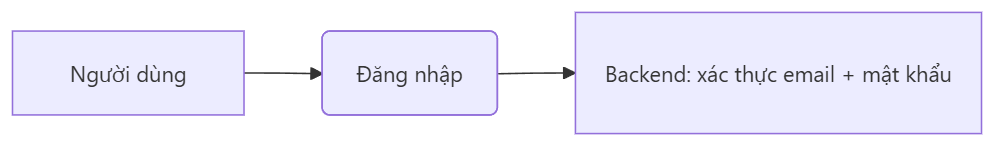
\includegraphics[width=\textwidth]{images/image7.png}
    \caption{Giao diện Chi tiết Tuyến và Dòng thời gian Trạm dừng}
\end{figure}

Một thành phần nổi bật trong giao diện này là dải Dòng thời gian (Timeline) hiển thị thứ tự các trạm mà tuyến xe đi qua. Đồng thời, hệ thống cung cấp tính năng Xem đánh giá (Reviews), nơi hành khách có thể để lại bình chọn 1-5 sao và nhận xét cá nhân về chất lượng phục vụ của tuyến.

\section{Nhóm công cụ Phân tích Không gian (GIS Tools)}

\subsection{Tra cứu và tìm hướng đi định tuyến (Routing)}

Tính năng cốt lõi giúp phân biệt BusGIS với các website tra cứu thông thường là công cụ định tuyến tự động. Bằng cách chọn điểm xuất phát và điểm đến trên bản đồ, công cụ tính toán sẽ sử dụng thuật toán phân tích mạng lưới tuyến để đề xuất lộ trình phù hợp, bao gồm các điểm trung chuyển nếu cần chuyển tuyến.

\begin{figure}[H]
    \centering
    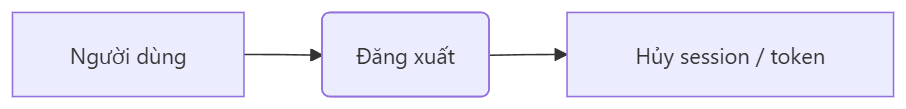
\includegraphics[width=\textwidth]{images/image8.png}
    \caption{Công cụ Tìm kiếm Định tuyến xe buýt}
\end{figure}

Kết quả được vẽ trực tiếp bằng các dải màu nổi bật trên bản đồ không gian, kèm theo bảng hướng dẫn di chuyển chi tiết từng chặng phía bên lề trái màn hình.

\subsection{Đánh giá không gian mạng lưới dịch vụ (Buffer Zone)}

Chức năng tạo vùng đệm (Buffer Zone) cho phép phân tích phạm vi bao phủ của mạng lưới giao thông. Người dùng chọn một trạm dừng và thiết lập bán kính (ví dụ 500m hoặc 1km), hệ thống sẽ vẽ một vòng tròn bao quanh trạm trên bản đồ.

\begin{figure}[H]
    \centering
    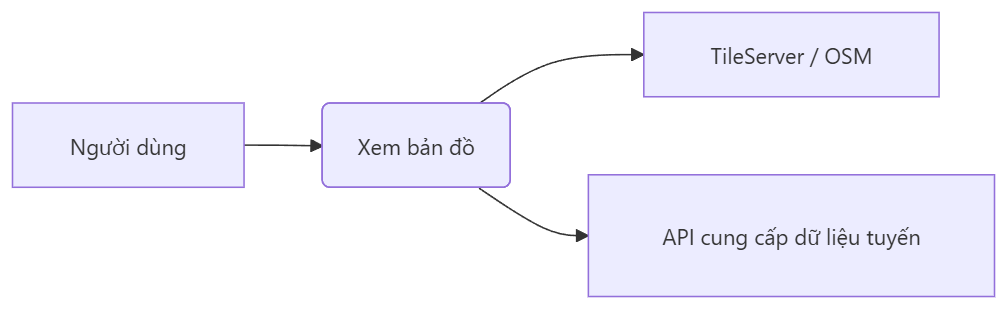
\includegraphics[width=\textwidth]{images/image9.png}
    \caption{Phân tích vùng đệm phục vụ của Trạm xe buýt}
\end{figure}

Tính năng này hỗ trợ đắc lực trong việc đánh giá mức độ tiếp cận giao thông công cộng tại khu vực cư dân cụ thể, hỗ trợ công tác quy hoạch điểm đặt trạm mới cho cơ quan quản lý.

\section{Phân hệ Xác thực hệ thống và Chiến lược Bảo mật}

Hệ thống BusGIS quản lý quyền truy cập thông qua mô hình phân quyền chặt chẽ. Trang Đăng nhập (Login) và Đăng ký (Register) được thiết kế hiện đại, thông báo lỗi rõ ràng. 

\begin{figure}[H]
    \centering
    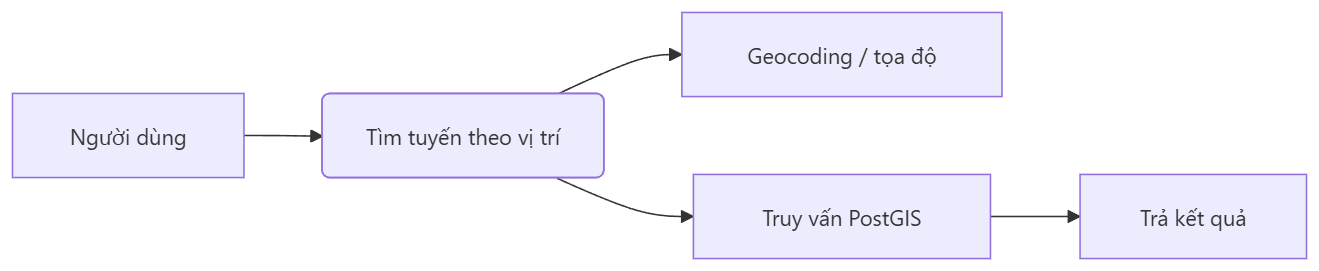
\includegraphics[width=\textwidth]{images/image10.png}
    \caption{Giao diện Xác thực người dùng}
\end{figure}

Sau khi xác thực, người dùng sở hữu không gian Quản lý Hồ sơ cá nhân (Profile) để cập nhật thông tin. Đặc biệt đối với các tài khoản thuộc cấp Quản trị (Admin/Staff), hệ thống tự động mở khóa liên kết đến Bảng điều khiển Quản lý nội bộ (Management Dashboard). Tại đây, quản trị viên có thể giám sát số lượng tài khoản đăng ký mới, thực hiện thêm/sửa/xóa tuyến xe và xuất báo cáo dữ liệu định dạng Excel.

\chapter{ĐÁNH GIÁ CHẤT LƯỢNG HỆ THỐNG}

\section{Đánh giá thiết kế Giao diện và Trải nghiệm người dùng}

Kết quả thực nghiệm cho thấy phân hệ giao diện tương tác của BusGIS đã đáp ứng tốt các tiêu chí về thiết kế UI/UX (User Interface / User Experience). Giao diện được xây dựng theo phong cách hiện đại, sử dụng bảng màu tương phản giúp người dùng dễ dàng nhận diện các nút chức năng và thông tin quan trọng. Hệ thống đảm bảo tính tương thích (Responsive) trên đa dạng các thiết bị, từ màn hình máy tính bàn, máy tính bảng cho đến điện thoại di động mà không gây vỡ cấu trúc hay mất mát dữ liệu. 

Bản đồ nền (Basemap) tích hợp từ LeafletJS tải mượt mà, thao tác vuốt, thu phóng diễn ra trơn tru ngay cả khi mạng lưới phải hiển thị đồng thời hàng trăm trạm dừng. Các tính năng hướng dẫn thao tác, thông báo lỗi (ví dụ khi tìm kiếm không có kết quả, đăng nhập sai mật khẩu) được xử lý thông qua các cảnh báo Toast tinh tế, mang lại trải nghiệm sử dụng chuyên nghiệp. Đặc biệt, việc bổ sung hệ thống đánh giá (Review) tạo không gian tương tác hai chiều, giúp người quản trị lắng nghe trực tiếp phản hồi từ phía hành khách.

\section{Đánh giá Kết quả Phân tích chức năng lõi}

Nhóm công cụ phân tích không gian (GIS Tools) – trái tim của hệ thống, hoạt động đạt hiệu quả cao với độ chính xác số liệu đáng tin cậy.

\begin{itemize}
    \item \textbf{Khả năng định tuyến (Routing Engine):} Thuật toán tìm đường hoạt động ổn định. Khi người dùng nhập địa điểm đi và đến, hệ thống nhanh chóng phân tích và thiết lập đồ thị không gian mạng lưới, trả về danh sách các tuyến xe buýt liên quan. Quá trình tính toán trên Backend diễn ra nhanh, các đường vẽ lộ trình (Polyline) trên bản đồ khớp nối chính xác với địa hình giao thông thực tế.
    \item \textbf{Tra cứu bán kính không gian (Buffer Query):} Công cụ tìm trạm gần nhất và xác định vùng đệm dựa trên thuật toán Haversine đem lại kết quả chuẩn xác. Việc ứng dụng cấu trúc lưu trữ dữ liệu Point của PostGIS đã giúp tối ưu hóa thời gian quét dữ liệu, cho phép lọc hàng ngàn trạm xe buýt và chỉ trả về những trạm nằm trong giới hạn bán kính được người dùng chỉ định.
\end{itemize}

\section{Đánh giá cơ chế Phân quyền và Hiệu năng}

Cơ chế phân quyền được thực thi nghiêm ngặt thông qua thư viện Authentication mặc định của Django. Hệ thống phân chia rõ ràng ranh giới giữa chức năng công cộng (Guest), chức năng thành viên (User) và quản trị viên (Admin/Staff). Việc bảo mật các API cập nhật dữ liệu (Thêm, Sửa, Xóa) thông qua token CSRF ngăn chặn hiệu quả các hình thức tấn công giả mạo yêu cầu.

Về mặt hiệu năng, quá trình tải dữ liệu bản đồ diện rộng được cải thiện đáng kể nhờ chiến lược phân trang (Pagination) ở tầng Backend. Thay vì gửi toàn bộ hàng nghìn trạm dừng cùng lúc, hệ thống chỉ phản hồi các gói dữ liệu nhỏ theo yêu cầu hiển thị của khung nhìn bản đồ, từ đó giảm áp lực băng thông mạng và tiết kiệm tài nguyên bộ nhớ trên thiết bị của người dùng.

\section{Các ưu điểm đạt được của đề tài}

Trải qua quá trình nghiên cứu và xây dựng, đề tài đã đạt được các thành quả đáng ghi nhận:
\begin{itemize}
    \item Số hóa thành công toàn bộ mạng lưới tuyến xe buýt và vị trí tọa độ các trạm dừng trên địa bàn thử nghiệm vào một hệ quản trị cơ sở dữ liệu không gian tập trung.
    \item Cung cấp hệ sinh thái tính năng hoàn thiện từ tra cứu thông tin cơ bản đến phân tích, định tuyến không gian phức tạp.
    \item Xây dựng trang Quản trị (Dashboard) chuyên nghiệp, hỗ trợ Import/Export dữ liệu Excel thuận tiện.
    \item Kiến trúc mã nguồn mở gọn nhẹ, linh hoạt, dễ dàng mở rộng và tích hợp thêm các dịch vụ bản đồ bên thứ ba trong tương lai.
\end{itemize}

\section{Các hạn chế còn tồn đọng}

Bên cạnh những kết quả tích cực, hệ thống vẫn còn một số điểm giới hạn cần được khắc phục:
\begin{itemize}
    \item Dữ liệu giao thông hiện tại mang tính tĩnh (Static Data), chưa tích hợp được công nghệ theo dõi vị trí GPS thời gian thực (Real-time Tracking) của các phương tiện đang di chuyển trên tuyến.
    \item Thuật toán định tuyến trung chuyển (chuyển qua 2-3 tuyến xe khác nhau) chưa tính toán được các rào cản giao thông thực tế như mật độ kẹt xe, đường cấm theo giờ.
    \item Dữ liệu nguồn từ OpenStreetMap đôi khi vẫn còn thiếu sót về các tiện ích chi tiết tại trạm dừng (ví dụ: thông tin bãi đỗ xe máy kế cận, nhà vệ sinh công cộng).
\end{itemize}

\chapter{KẾT LUẬN VÀ HƯỚNG PHÁT TRIỂN TƯƠNG LAI}

\section{Tổng kết và ý nghĩa thực tiễn của đề tài}

Đề tài "Hệ thống WebGIS quản lý và tra cứu tuyến xe buýt thông minh (BusGIS)" đã đi sâu nghiên cứu và ứng dụng thành công các công nghệ thông tin địa lý vào lĩnh vực giao thông vận tải. Sản phẩm đầu ra không chỉ đơn thuần là một website thông tin mà là một hệ thống bản đồ số tương tác (WebGIS) toàn diện, bao gồm cả phân hệ quản lý dữ liệu không gian phức tạp và phân hệ phân tích địa lý trực quan cho người dùng cuối. 

Việc chuyển đổi từ phương pháp quản lý, tra cứu thủ công sang hệ thống bản đồ số trực tuyến mang lại nhiều ý nghĩa thiết thực. Đối với người dân, hệ thống giúp tiết kiệm thời gian, tăng cường mức độ chủ động trong việc lựa chọn phương tiện giao thông công cộng, từ đó góp phần giảm thiểu sử dụng xe cá nhân, giảm ùn tắc giao thông và bảo vệ môi trường. Đối với cơ quan quản lý nhà nước và doanh nghiệp vận tải, BusGIS cung cấp một nền tảng số hóa tập trung, hỗ trợ lưu trữ an toàn, theo dõi phản hồi hành khách và ra quyết định tối ưu hóa mạng lưới trạm tuyến dựa trên bằng chứng dữ liệu không gian trực quan.

Toàn bộ đồ án đã hoàn thành các mục tiêu ban đầu đề ra: ứng dụng thành thạo PostgreSQL/PostGIS trong việc tổ chức mô hình dữ liệu địa lý, khai thác mạnh mẽ framework Django cho kiến trúc Backend và xây dựng giao diện hiển thị không gian sinh động qua LeafletJS. Quá trình thực hiện đề tài đã giúp củng cố kiến thức nền tảng về hệ thống thông tin địa lý, đồng thời nâng cao kỹ năng lập trình và khả năng giải quyết các bài toán thực tiễn.

\section{Đề xuất hướng mở rộng và phát triển tương lai}

Dựa trên những nền tảng đã xây dựng, hệ thống BusGIS sở hữu tiềm năng rất lớn để mở rộng và nâng cấp trong tương lai nhằm đáp ứng nhu cầu giao thông thông minh (Smart Mobility) của một đô thị hiện đại. Một số định hướng phát triển cụ thể bao gồm:

\begin{itemize}
    \item \textbf{Tích hợp hệ thống theo dõi thời gian thực (Real-time GPS Tracking):} Lắp đặt hoặc kết nối với hệ thống định vị trên các xe buýt đang vận hành để hiển thị vị trí thực tế của xe trên bản đồ. Tính năng này sẽ giúp hành khách ước tính chính xác thời gian xe đến trạm, cải thiện đáng kể trải nghiệm người dùng.
    \item \textbf{Phát triển ứng dụng trên thiết bị di động (Mobile App):} Chuyển đổi và đóng gói nền tảng WebGIS hiện tại thành ứng dụng Native (iOS/Android) hoặc PWA (Progressive Web App) để tận dụng các phần cứng di động như la bàn, GPS, thông báo đẩy (Push Notifications), giúp người dùng tra cứu thuận tiện mọi lúc mọi nơi.
    \item \textbf{Ứng dụng Trí tuệ nhân tạo (AI) và Phân tích Dữ liệu Lớn (Big Data):} Thu thập dữ liệu tìm kiếm, lưu lượng truy cập và đánh giá của người dùng để dự đoán các điểm nóng giao thông, phân tích nhu cầu đi lại theo giờ cao điểm. Từ đó đề xuất cho ban quản lý mở thêm tuyến mới hoặc điều chỉnh tần suất chuyến.
    \item \textbf{Tích hợp đa phương thức giao thông (Multi-modal Routing):} Nâng cấp thuật toán định tuyến để kết hợp xe buýt với các phương tiện công cộng khác như tàu điện ngầm (Metro), xe đạp công cộng hoặc xe ôm công nghệ (Ride-hailing), cung cấp lộ trình di chuyển xuyên suốt cho hành khách từ cửa nhà đến đích đến.
    \item \textbf{Bổ sung tính năng tương tác cộng đồng:} Cho phép người dùng báo cáo trực tiếp sự cố giao thông (kẹt xe, ngập nước, tai nạn) lên bản đồ theo thời gian thực để hệ thống tự động tính toán lại lộ trình và cảnh báo cho các hành khách khác đang có dự định đi qua khu vực đó.
\end{itemize}

Việc tiếp tục nghiên cứu và hoàn thiện các tính năng trên sẽ đưa BusGIS trở thành một hệ sinh thái giao thông công cộng mạnh mẽ, góp phần đắc lực vào công cuộc chuyển đổi số và xây dựng đô thị thông minh (Smart City) tại Việt Nam.


\end{document}
